\documentclass[journal,letterpaper]{IEEEtran}
\usepackage[letterpaper, left=0.65in, right=0.65in, bottom=0.7in, top=0.7in]{geometry}
\usepackage{stix}
\usepackage{siunitx}
\usepackage[version=4]{mhchem}
\usepackage{booktabs}
\usepackage{makecell}
\usepackage{multirow}
\usepackage{amsmath}
\usepackage{bm}
\usepackage{graphicx}
\usepackage{tikz}
\usepackage{pgfplots}
\usepackage{float}
\usepackage{fancyhdr}
\usepackage[none]{hyphenat}
\usepackage[hidelinks]{hyperref}
\usepackage{import}
\usepackage{transparent}
\usepackage{microtype}

\graphicspath{ {./figures/} }

\pgfplotsset{compat=1.18}

\setlength{\columnsep}{0.2in}
\setlength{\columnwidth}{3.5in}

\newlength\fheight
\newlength\fwidth
\setlength\fwidth{3.25in}
\setlength\fheight{0.8\fwidth}

\newcommand{\incfig}[1]{%
    \centering
    \def\svgwidth{3.5in}
    \import{./figures/}{#1.pdf_tex}
}

\renewcommand{\arraystretch}{1.3}

\sisetup{per-mode = symbol,
         inter-unit-product = \ensuremath{ { } \cdot { } },
         number-unit-product = \text{ },
         group-digits = false,
         detect-weight = true,
         detect-inline-weight = math,
         detect-display-math = true}

\pagestyle{fancy}
\fancyhf{}
\renewcommand{\headrulewidth}{0pt}
\rhead{\thepage}
\lhead{Section 11832 Lab 5}

\begin{document}
\title{Comparing NACA0012 Characteristics Using Pressure Taps in a Wind Tunnel}

\author{\IEEEauthorblockN{\LARGE{Borg, Auston J. \quad Lam, Brandon H. \quad Latzko, Alexander J. \\}}
\IEEEauthorblockA{
Section 11832 \quad October 31, 2023}
}

\maketitle
\thispagestyle{empty}

\begin{abstract}

\end{abstract}

\begin{IEEEkeywords}

\end{IEEEkeywords}


\section{Introduction}


\IEEEPARstart{I}{ntro}


\section{Procedure}

\subsection{s1}

\begin{figure}[H]
    \centering
    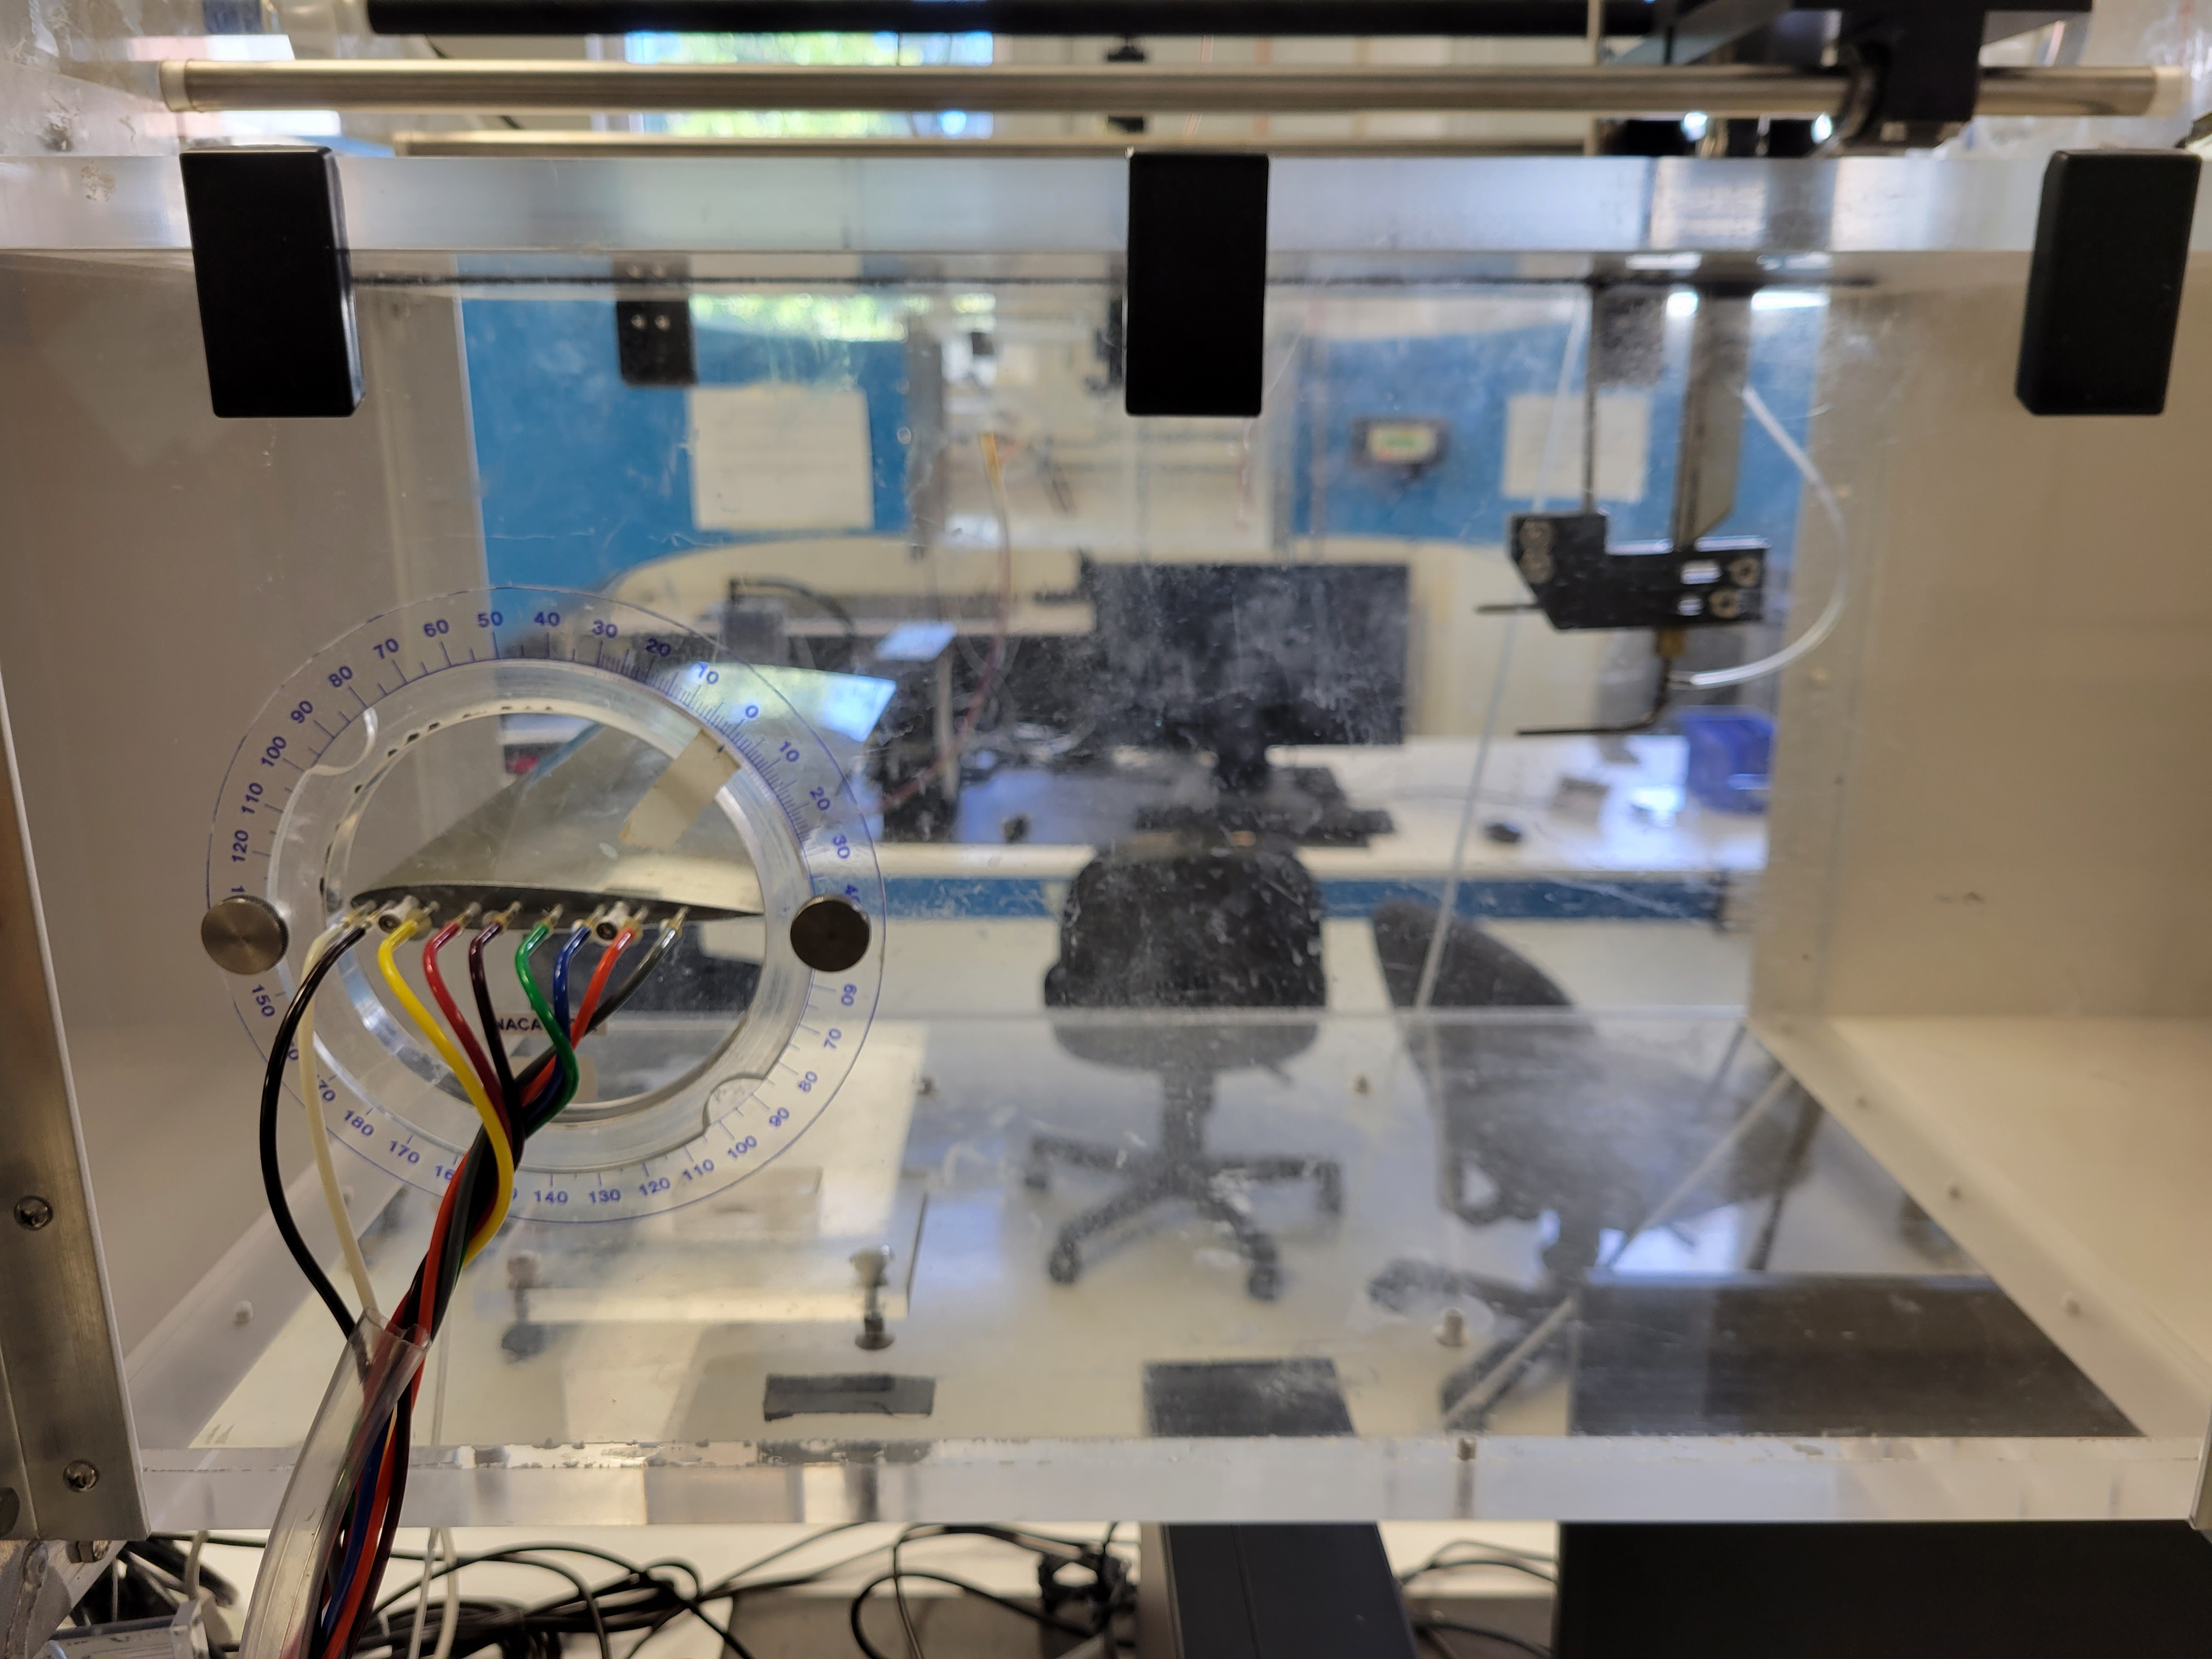
\includegraphics[width=3.5in]{testSection}
    \caption{Wind tunnel test section with NACA0012 airfoil installed. The airfoil is oriented at an angle of attack of zero degrees.}
    \label{fig:section}
\end{figure}


\section{Results}


The ambient pressure, $P_\text{amb}$, of the room was measured using a wall-mounted barometer.
The temperature, $T$, and the relative humidity, $\varphi$, of the room was measured using a digital thermometer and hygrometer placed next to the test section.
The measured atmospheric conditions are summarized in Table~\ref{tab:atmCond}.

\begin{table}[H]
    \centering
    \caption{Atmospheric Conditions}
    \renewcommand{\arraystretch}{1.105}
    \begin{tabular}{ccc}
    \toprule
    Parameter & Value & Uncertainty ($\pm$) \\ \midrule \midrule
    $P_\text{amb}$ & \qty{767.70}{mm\ce{Hg}} & \qty{0.02}{mm\ce{Hg}} \\
    $T$ & \qty{21.1}{\celsius} & \qty{0.1}{\celsius} \\
    $\varphi$ & 49\% & 1\% \\ \bottomrule
    \end{tabular}
    \label{tab:atmCond}
\end{table}

\begin{figure}[H]
    \centering
    %\input{figures/cal.tex}
    \caption{Hot wire anemometer calibration curve.}
    \label{fig:cal}
\end{figure}


\section{Discussion}


\begin{figure}[H]
    \centering
    %% This file was created by matlab2tikz.
%
%The latest updates can be retrieved from
%  http://www.mathworks.com/matlabcentral/fileexchange/22022-matlab2tikz-matlab2tikz
%where you can also make suggestions and rate matlab2tikz.
%
\definecolor{mycolor1}{rgb}{0.00000,0.44700,0.74100}%
\definecolor{mycolor2}{rgb}{0.98039,0.27451,0.08627}%
\definecolor{mycolor3}{rgb}{0.85000,0.32500,0.09800}%
\definecolor{mycolor4}{rgb}{0.00000,0.12941,0.64706}%
%
\begin{tikzpicture}

\begin{axis}[%
width=0.958\fwidth,
height=\fheight,
at={(0\fwidth,0\fheight)},
xmin=-2,
xmax=14,
xlabel style={font=\color{white!15!black}\small},
xlabel={Angle of Attack (deg)},
ymin=-0.05,
ymax=0.25,
yticklabel style={
            /pgf/number format/fixed,
            /pgf/number format/precision=2,
            /pgf/number format/fixed zerofill
        },
ylabel style={font=\color{white!15!black}\small},
ylabel={$C_D$},
ytick={-0.05,0,...,0.25},
axis background/.style={fill=white},
axis x line*=bottom,
axis y line*=left,
xmajorgrids,
ymajorgrids,
tick label style={font=\small},
legend style={at={(0.03,0.97)}, anchor=north west, legend cell align=left, align=left, draw=white!15!black, font=\footnotesize}
]
\addplot [color=black, only marks, mark=triangle*, mark options={solid, fill=mycolor2, draw=mycolor2}]
plot [error bars/.cd, x dir=both, x explicit, y dir=both, y explicit, error bar style={line width=0.5pt}, error mark options={line width=0.5pt, mark size=3.0pt, rotate=90}]
table[row sep=crcr, y error index=2, x error index=3]{%
0	0.024098266	0.01	0.1\\
3	0.02097669	0.012	0.1\\
5	0.019603469	0.014	0.1\\
7	0.022362807	0.017	0.1\\
8	0.032307843	0.019	0.1\\
9	0.061423923	0.021	0.1\\
10	0.070496385	0.023	0.1\\
11	0.123933934	0.026	0.1\\
12	0.162515846	0.028	0.1\\
13	0.180300215	0.03	0.1\\
};
\addlegendentry{Uncorrected}

\addplot [color=black, only marks, mark=square*, mark options={solid, fill=mycolor4, draw=mycolor4}]
plot [error bars/.cd, x dir=both, x explicit, y dir=both, y explicit, error bar style={line width=0.5pt}, error mark options={line width=0.5pt, mark size=3.0pt, rotate=90}]
table[row sep=crcr, y error index=2, x error index=3]{%
0	0.023524806	0.01	0.1\\
3.051219576	0.020477514	0.012	0.1\\
5.083739423	0.019136971	0.014	0.1\\
7.117555465	0.021830646	0.017	0.1\\
8.140641138	0.031539023	0.019	0.1\\
9.173948407	0.059962236	0.021	0.1\\
10.19552088	0.068818803	0.023	0.1\\
11.17868962	0.120984715	0.026	0.1\\
12.17634195	0.158648504	0.028	0.1\\
13.1769283	0.176009664	0.03	0.1\\
};
\addlegendentry{Corrected}

\addplot [color=black, line width=1.2pt]
  table[row sep=crcr]{%
0	0.008842244\\
0.05	0.008839894\\
0.1	0.008842193\\
0.15	0.008848226\\
0.2	0.008853654\\
0.25	0.008862198\\
0.3	0.008866107\\
0.35	0.008878755\\
0.4	0.008894147\\
0.45	0.008904845\\
0.5	0.008914627\\
0.55	0.008936335\\
0.6	0.008956403\\
0.65	0.008970107\\
0.7	0.008987954\\
0.75	0.009013733\\
0.8	0.009038003\\
0.85	0.009060692\\
0.9	0.009078774\\
1	0.009138079\\
1.05	0.009166962\\
1.1	0.009193608\\
1.15	0.009218441\\
1.2	0.009252837\\
1.25	0.009284323\\
1.3	0.009317042\\
1.35	0.009349723\\
1.4	0.009375954\\
1.45	0.009413921\\
1.5	0.009445401\\
1.55	0.0094814\\
1.6	0.009514411\\
1.65	0.009547555\\
1.7	0.009583161\\
1.75	0.009614014\\
1.8	0.009653574\\
1.85	0.009682475\\
1.9	0.009723635\\
1.95	0.009752705\\
2	0.00979463\\
2.05	0.009823753\\
2.1	0.00986176\\
2.15	0.009892156\\
2.2	0.009931544\\
2.25	0.009964881\\
2.3	0.01000745\\
2.35	0.01003672\\
2.4	0.01007481\\
2.45	0.01010592\\
2.5	0.01014927\\
2.55	0.01018592\\
2.6	0.01022726\\
2.65	0.01025297\\
2.7	0.01029726\\
2.75	0.01032646\\
2.8	0.01037541\\
2.85	0.01040184\\
2.9	0.01043647\\
2.95	0.01047335\\
3	0.01051069\\
3.05	0.01055327\\
3.1	0.01057927\\
3.15	0.0106249\\
3.2	0.01064561\\
3.25	0.01068194\\
3.3	0.01070268\\
3.35	0.01074377\\
3.4	0.01076468\\
3.5	0.01083134\\
3.55	0.01087682\\
3.6	0.01090314\\
3.65	0.01095069\\
3.7	0.01097975\\
3.75	0.01102941\\
3.8	0.01106126\\
3.85	0.01111418\\
3.9	0.0111482\\
4	0.01124038\\
4.05	0.01130053\\
4.1	0.01133826\\
4.15	0.01139919\\
4.2	0.0114428\\
4.25	0.01150394\\
4.3	0.0115539\\
4.35	0.01161466\\
4.4	0.01167191\\
4.45	0.01173192\\
4.5	0.01179726\\
4.55	0.01185614\\
4.6	0.0119304\\
4.65	0.01198779\\
4.7	0.01206803\\
4.75	0.01212793\\
4.8	0.01220521\\
4.85	0.01227707\\
4.9	0.01235131\\
4.95	0.01243529\\
5	0.01250634\\
5.05	0.01260047\\
5.1	0.01267079\\
5.15	0.01276157\\
5.2	0.01284501\\
5.25	0.01293259\\
5.3	0.0130283\\
5.35	0.0131127\\
5.4	0.01321908\\
5.45	0.01330059\\
5.55	0.01349509\\
5.6	0.0136133\\
5.65	0.01369547\\
5.75	0.01390104\\
5.8	0.01402119\\
5.85	0.01411256\\
5.9	0.01422475\\
5.95	0.0143343\\
6	0.01443383\\
6.05	0.01457139\\
6.1	0.01465546\\
6.15	0.01476793\\
6.2	0.01490256\\
6.25	0.01498909\\
6.3	0.01510558\\
6.35	0.0152491\\
6.4	0.01533456\\
6.45	0.01544372\\
6.5	0.01559304\\
6.55	0.01569818\\
6.6	0.01579824\\
6.65	0.01591692\\
6.7	0.01608482\\
6.75	0.01617772\\
6.8	0.01627857\\
6.85	0.01639316\\
6.9	0.01654853\\
6.95	0.01668227\\
7	0.01677888\\
7.05	0.01688917\\
7.1	0.0170133\\
7.15	0.01717906\\
7.2	0.01732791\\
7.25	0.01743044\\
7.3	0.01754511\\
7.35	0.0176662\\
7.4	0.01780327\\
7.45	0.01798922\\
7.5	0.01813876\\
7.55	0.01824234\\
7.6	0.01835812\\
7.65	0.01848035\\
7.7	0.01861158\\
7.75	0.01876919\\
7.8	0.01899887\\
7.85	0.01910988\\
7.9	0.01922461\\
7.95	0.01935129\\
8	0.01948438\\
8.05	0.01962478\\
8.1	0.01977829\\
8.15	0.01996249\\
8.2	0.02021514\\
8.25	0.02037036\\
8.3	0.02049893\\
8.35	0.02063909\\
8.4	0.02078274\\
8.45	0.02092712\\
8.5	0.02107409\\
8.55	0.02122949\\
8.6	0.02140845\\
8.65	0.02164574\\
8.7	0.02189836\\
8.75	0.02202152\\
8.8	0.02216307\\
8.85	0.02231325\\
8.9	0.0224671\\
8.95	0.02262289\\
9	0.02278211\\
9.05	0.02294887\\
9.1	0.02313233\\
9.15	0.02334666\\
9.2	0.02362176\\
9.25	0.02395172\\
9.3	0.02411333\\
9.35	0.02429577\\
9.4	0.0244903\\
9.45	0.02468998\\
9.5	0.02488863\\
9.55	0.02508378\\
9.6	0.02527451\\
9.65	0.02546198\\
9.7	0.02564787\\
9.75	0.0258369\\
9.8	0.02603905\\
9.85	0.02627417\\
9.9	0.02658444\\
9.95	0.02699279\\
10	0.02716623\\
10.05	0.02736571\\
10.1	0.02758027\\
10.15	0.02780166\\
10.2	0.02802418\\
10.25	0.02824478\\
10.3	0.02846326\\
10.35	0.028683\\
10.4	0.02890294\\
10.45	0.02912592\\
10.5	0.02935482\\
10.55	0.02958806\\
10.6	0.02983083\\
10.65	0.03009423\\
10.7	0.03039673\\
10.75	0.03077617\\
10.8	0.03132593\\
10.85	0.03162793\\
10.9	0.0319185\\
10.95	0.03223135\\
11	0.03256163\\
11.05	0.03290512\\
11.1	0.03325831\\
11.15	0.03361811\\
11.2	0.03398107\\
11.25	0.03434205\\
11.3	0.03469854\\
11.35	0.03504835\\
11.4	0.03538945\\
11.45	0.03571975\\
11.5	0.03603764\\
11.55	0.0363413\\
11.6	0.03662947\\
11.65	0.03690166\\
11.7	0.03718142\\
11.75	0.03746024\\
11.8	0.0377363\\
11.85	0.03801663\\
11.9	0.03831214\\
11.95	0.03863848\\
12	0.03903101\\
12.05	0.03957446\\
12.1	0.04026817\\
12.15	0.04064883\\
12.2	0.04103006\\
12.25	0.04142497\\
12.3	0.04184196\\
12.35	0.04228231\\
12.4	0.04274592\\
12.45	0.04323177\\
12.5	0.0437387\\
12.55	0.04426629\\
12.6	0.04481405\\
12.65	0.04538244\\
12.7	0.04597117\\
12.75	0.04658202\\
12.8	0.04721482\\
12.85	0.04787097\\
12.9	0.04855086\\
12.95	0.04925354\\
13	0.04998036\\
};
\addlegendentry{XFLR5}

\end{axis}
\end{tikzpicture}%
    \caption{Calibration graph for voltage velocity relation.}
    \label{fig:calCurve}
\end{figure}


\section{Conclusion}





\section*{Appendix A: Uncertainty Calculations}


\begin{table}[H]
    \renewcommand{\arraystretch}{1.7}
    \centering
    \caption{Summary of Measurement Uncertainties}
    \begin{tabular}{cccc}
    \toprule
    Parameter & Symbol & Justification & Uncertainty ($\pm$) \\ \midrule \midrule
    Temperature & $\mu T$ & Digital & \qty{0.1}{\celsius} \\
    Humidity & $\mu \varphi$ & Digital & 1\% \\
    Ambient Pressure & $\mu P_\text{amb}$ & Barometer & \qty{0.02}{\mm} \\
    \makecell{Static Pressure \\ Difference} & $\mu \Delta P$ & \makecell{95\% Conf. Int.} & Variable \\
    Voltage & $\mu V$ & 95\% Conf. Int. & Variable \\
    Dynamic Pressure & $\mu q$ & RSS & Variable \\
    Saturation Pressure & $\mu P_g$ & RSS & \qty{16}{\pascal} \\
    Density & $\mu \rho$ & RSS & \qty{0.004}{\kg\per\m\cubed} \\
    Calibration Velocity & $\mu v_c$ & RSS & $\sim \qty{0.04}{\m\per\s}$ \\
    Interpolated Velocity & $\mu v$ & \makecell{Largest \\ Percent Error} & 0.5\% \\
    Freestream Velocity & $\mu U_\infty$ & RSS & \qty{0.04}{\m\per\s} \\
    Characteristic Length & $\mu L$ & Ruler & \qty{0.5}{\mm} \\
    Kinematic Viscosity & $\mu \nu$ & \cite{HeatTrans} & \qty{2e-9}{\m\squared\per\s} \\
    Reynolds Number & $\mu Re$ & RSS & 938 \\
    Height & $\mu h$ & Ruler & \qty{0.05}{\cm} \\
    Instantaneous Velocity & $\mu U_2$ & 95\% Conf. Int. & Variable \\
    Drag Force & $\mu F_D$ & RSS & \qty{0.070}{\newton} \\
    Coefficient of Drag & $\mu v$ & RSS & 0.065 \\ \bottomrule
    \end{tabular}
    \label{tab:uncertainty}
\end{table}

The uncertainties for each measured value are summarized in Table~\ref{tab:uncertainty}.
First, the systemic bias in the reading of the transducer pressures and the voltage readings was accounted for by zeroing the respective values in the LabVIEW VI.
The random uncertainty for each reading was then obtained by using a 95\% confidence interval with a normal distribution.
Because a sample size of 20000 was used for each reading, it was determined to be sufficiently large that the sample distribution approached the normal distribution according to the central limit theorem~\cite{MoMLecture}.
A $z^*$ value of 1.96 was used for the calculation of the 95\% confidence interval~\cite{MoMLecture}.
The margin of error then served as the uncertainty as seen in~\eqref{eq:conf}, where $\mu X$ is the margin of error for an arbitrary measurement, $S_x$ is the sample standard deviation, and $n$ is the number of samples~\cite{MoMLecture}.

\begin{equation} \label{eq:conf}
    \mu X = z^* \frac{S_x}{\sqrt{n}}
\end{equation}

The uncertainties in the calculated dynamic pressures, $q$, were then calculated using the root sum squared (RSS) method as seen in~\eqref{eq:uq}, where $\Delta P$ is the change in stagnation pressure and $k$ is the tunnel calibration coefficient that was determined in the first lab experiment~\cite{MoMLecture}.

\begin{equation} \label{eq:uq}
    \mu q = \left[\left(\mu \Delta P \frac{\partial q}{\partial \Delta P}\right)^2 + \left(\mu k \frac{\partial q}{\partial k}\right)^2\right]^{1/2}
\end{equation}

The uncertainty in the saturation pressure, $P_g$, was determined using error propagation theory as seen in~\eqref{eq:uPsat}, where $T$ is the ambient temperature~\cite{errorprop}.

\begin{equation} \label{eq:uPsat}
    \mu P_g = \mu T \frac{\partial P_g}{\partial T}
\end{equation}

The uncertainty in the fluid density, $\rho$, was calculated using the RSS method as seen in~\eqref{eq:uRho}, where $P$ is the ambient pressure, $T$ is the ambient temperature, $\varphi$ is the relative humidity, and $P_g$ is the saturation pressure~\cite{MoMLecture}.

\begin{equation} \label{eq:uRho}
    \resizebox{227pt}{!}{$\displaystyle{\mu \rho = \left[\left(\mu P \frac{\partial \rho}{\partial P}\right)^2 + \left(\mu T \frac{\partial \rho}{\partial T}\right)^2 + \left(\mu \varphi \frac{\partial \rho}{\partial \varphi}\right)^2 + \left(\mu P_g \frac{\partial \rho}{\partial P_g}\right)^2\right]^{1/2}}$}
\end{equation}

The uncertainty for the fluid velocity used in the calibration of the hot wire anemometer, $v_c$, was then calculated using the RSS method as seen in~\eqref{eq:uv}, where $q$ is the dynamic pressure, $\rho$ is the fluid density, and $V$ is voltage from the hot wire anemometer obtained from the fourth-order polynomial fit~\cite{MoMLecture}.

\begin{equation} \label{eq:uv}
    \mu v_c = \left[\left(\mu q \frac{\partial v_c}{\partial q}\right)^2 + \left(\mu \rho \frac{\partial v_c}{\partial \rho}\right)^2 + \left(\mu V \frac{\partial v_c}{\partial V}\right)^2\right]^{1/2}
\end{equation}

Then, to obtain the uncertainty for the interpolated fluid velocities, $v$, the greatest percent error from the calibration of the hot wire anemometer was used to simulate the worst-case deviation for all the interpolated velocities using the calibration curve.

The uncertainty for the Reynolds number, $Re$, was calculated using the RSS method as seen in~\eqref{eq:uRe}, where $U_\infty$ is the freestream velocity, $\nu$ is the dynamic viscosity of the fluid, and $L$ is the characteristic length~\cite{HeatTrans}.

\begin{equation} \label{eq:uRe}
    \resizebox{227pt}{!}{$\displaystyle{\mu Re = \left[\left(\mu \nu \frac{\partial Re}{\partial \nu}\right)^2 + \left(\mu U_\infty \frac{\partial Re}{\partial U_\infty}\right)^2 + \left(\mu L \frac{\partial Re}{\partial L}\right)^2\right]^{1/2}}$}
\end{equation}

To obtain the uncertainties for the instantaneous velocity, a 95\% confidence interval was used.
The sample size of the data was larger than 1000, so a normal distribution was used.
For a 95\% confidence interval, the corresponding $z^*$ value of 1.96 was used~\cite{MoMLecture}.
Using~\eqref{eq:conf}, the uncertainty in each velocity was found.

The uncertainty in the drag force, $F_D$, was calculated using the RSS method as seen in~\eqref{eq:uFD}, where $q$ is the dynamic pressure, $h$ is the height of the velocity profile, $U_2 (y)$ is the instantaneous velocity, and $U_\infty$ is the freestream velocity.

\begin{equation} \label{eq:uFD}
    \resizebox{227pt}{!}{$\displaystyle{\mu F_D = \left[\left(\mu U_\infty \frac{\partial F_D}{\partial U_\infty}\right)^2 + \left(\mu q \frac{\partial F_D}{\partial q}\right)^2 + \left(\mu h \frac{\partial F_D}{\partial h}\right)^2 + \left(\mu U_2 (y) \frac{\partial F_D}{\partial U_2 (y)}\right)^2\right]^{1/2}}$}
\end{equation}

The uncertainty in the drag coefficient, $C_D$, was calculated using the RSS method as seen in~\eqref{eq:uCD}, where $q$ is the dynamic pressure, $F_D$ is the drag force, and $L$ is the characteristic length.

\begin{equation} \label{eq:uCD}
    \resizebox{227pt}{!}{$\displaystyle{\mu C_D = \left[\left(\mu F_D \frac{\partial C_D}{\partial F_D}\right)^2 + \left(\mu q \frac{\partial C_D}{\partial q}\right)^2 + \left(\mu L \frac{\partial C_D}{\partial L}\right)^2\right]^{1/2}}$}
\end{equation}

\noindent
This lab report was typeset using \LaTeX.

\begin{thebibliography}{99}
    \bibitem{HeatTrans} Bergman, T. L., and Lavine, A. S., ``Appendix A: Thermophysical Properties of Matter,'' \textit{Fundamentals of Heat and Mass Transfer}, Wiley, Hoboken, NJ, 2017, p. 911.
    \bibitem{MoMLecture} Ridgeway, S., ``MOM\_lab Uncertainty basics w tension,'' \textit{University of Florida} [PowerPoint slides], URL: \url{https://ufl.instructure.com/courses/447927/files/65674680}, 2022.
    \bibitem{errorprop} Ku, H. H., ``Notes on the Use of Propagation of Error Formulas'', \textit{Journal of Research of the National Bureau of Standards}, Vol. 70C, No. 4, 27 May 1966, pp. 263--273.
\end{thebibliography}

\end{document}